\documentclass{article}
\usepackage[utf8]{inputenc}
\usepackage[english]{babel}
\usepackage{graphicx}
\usepackage{amsmath}
\usepackage{amssymb}
\usepackage{amsfonts}
\usepackage{amsthm}
\usepackage{subcaption}


\usepackage{biblatex}
\addbibresource{./bibli.bib}
\usepackage{hyperref}
\graphicspath{ {plots/} }
\hypersetup{
	linktocpage=true,
	colorlinks=true,
	linkcolor=red,
	filecolor=magenta,      
	urlcolor=cyan,
	pdftitle={Kelly's Criterion},
	pdfpagemode=FullScreen,
	bookmarks=true,
	breaklinks=true
}

\urlstyle{same}
\newtheorem{thm}{Theorem}[section]
\newtheorem{cor}[thm]{Corollary}
\newtheorem{lem}[thm]{Lemma}
\newcommand{\pdiv}[2]{{\frac{\partial#1}{\partial#2}}}

\title{Kelly's Criterion}
\date{2021-09-01}
\author{Eldad Kronfeld}


\begin{document}
	\maketitle
	\thanks{Thank you Hagai for the continuing patience and support along the way.}
	\tableofcontents
	\newpage
	\section{Abstract}
		This paper is about the mathematical model proposed by John Kelly \cite{Finance} at the early 1950s, 
		however instead of looking at the model from the lenses of games and gambles, each of our gamble is an option we can invest in until the next round of the model, at the beginning I will explain the basic concept behind the model and show simple example of a model with one investment with multiple outcomes, the results will be shown by using Monte Carlo simulations, later on I will expend the model to include multiple investments each with multiple outcomes with different possibilities.
	\section{The Base model}
	\subsection{Defining The Model}
	Kelly's Criterion is a model that runs till infinity (ideally) in discrete time frames, which I will call ticks$\backslash$rounds.
	The model represent a scenario where we gamble a fraction of our money each round and depending on what happens at the round we can win or loss money which would be our total amount for the next round.
	\newline
	However, the premise of the model is that the investments or gambles we take each round have expectations that are greater then 1,
	$$E_{gain} \ge 1$$
	meaning that in the long run we can expect that we will yield revenue from the ventures and not loss from it however because of the random nature of the model losses can happen.
	\newline
	\textbf{Note:} throughout all of the explanations and simulations I will normalize the results to be such as that we start with 1$\textdollar$ and each gain will be noted as $\gamma\cdot F_{N-1}$, where $F_{N-1}$ denotes the sum of money from round $N-1$ and $\gamma$ denotes the gain and $\gamma\in[0,\infty)$, so when $\gamma = 1$ it means that there is no gain and no loss at all, however when 
	$\gamma > 1$ we gain money and when $ 0\le \gamma < 1$ we can expect to loss money.
	\newline\newline
	if we try to define a simple model, where we have 1 investment with $k$ outcomes, where each outcome have $p_i$ probability of happening and we invest $f$ amount of money and keep $b=1-f$ 
		\begin{equation}
			\label{nes}
			F_N = \Bigg\{
			\begin{aligned}
				&(b + f\cdot \gamma _i)F_{N-1} &&N>1 \text{, for }i=1,..,k \\
				&1 &&for \enspace N=0
			\end{aligned}
		\end{equation}
	\\
	this equation represent our possible fortune at each round if we had $F_{N-1}$ before then. if outcome $i$ happens then the part that we didn't invest in $(1-f)$ doesn't change, however the part that we did invest $f$ changes by $\gamma_i$ meaning that we gained or lost some.
	\newline
	ultimately the way I looked at it, which helped me later to define more complicated model would be:\newline
	\textit{let} $X$ be random variable that represent the gain of each outcome, then for the outcome $\gamma_i$ the possibility of it happening is $P(X=\gamma_i) = p_i$, this will help us look at the exponential growth and develop a way to find the optimal fraction $f$ in each round to achieve the optimal returns.
	\\
	now let's look for the fraction \(f\) that produces the best gain, because of eq.\ref{nes} we can deduce that the growth rate from an investment is exponential because at each round we multiply our fortune:
	\begin{equation}
		\label{exp:FN}
		F_N = F_0e^{G_{N}N}
	\end{equation}
	so \(G_N = \frac{1}{N}log(\frac{F_N}{F_0}) = \sum_{i=1}^{k} \frac{W_i}{N}log(b + \gamma_i f)\), however when we take N to \(\infty\) in eq.\ref{exp:FN} we get the following equation:
	\begin{equation}
		\label{gain:func1}
		G = \lim_{N \to \infty} \sum_{i=1}^{k} \frac{W_i}{N}log(b+\gamma_i f) = \sum_{i=1}^{k} p_i log(b+\gamma_i f)
	\end{equation}
	then we would like to look for the maximum gain possible.
	\newline \newline
	\begin{thm}\label{thm1}
		$f(x) = -log(b(x)+\gamma x)$ is convex when $x\in (0,\infty)$, $b(x) = 1-x$.
	\end{thm}
	\begin{proof}
		$\pdiv{f}{x} = -\frac{\gamma - 1}{b+\gamma x}$ and the second derivative is 
		$\frac{\partial f}{\partial x^2} = \frac{(\gamma -1) ^2}{(b+\gamma x)^2}$\\
		second derivative is always positive, then $f(x)$ is convex.
		\newline
	\end{proof}	
	\begin{lem}
		\label{lem1}
		\(G(f) = \sum_{i=1}^{k} p_i log(b+\gamma_i f)\) is concave when $f\in (0,\infty)$, $b(f) = 1-f$.
	\end{lem}
	\begin{proof}
		when we look at eq.\ref{gain:func1} as a function of $f$,\\
		$G(f)$ is concave $\iff$ $-G(f)$ is convex.
		\[-G(f) = \sum_{i=1}^{k} p_i (-log(b+\gamma_i f))\]
		however a positive weighted sum of convex functions, is a convex function, each component $s_i = p_i log(b+\gamma_i f)$ is convex because $\gamma _i$ is non-negative , $0\le p_i \le 1$ and Theorem \ref{thm1} ,then \(-G(f)\) is convex, making $G(f)$ concave.
		\newline
	\end{proof}

	Because $G$ is concave, we will be able to find it's maximum by calculating the root of the Derivative, which is 
	\[\pdiv{G}{f} = \sum_{i=0}^{k} p_i \frac{\gamma_i - 1}{b+\gamma_i f} = 0\] 
	We know that a maxima exist inside $[0,1]$ because of last Lemma (\ref{lem1}), stating that $G(f)$ is concave making it's second derivative always non-positive, then the maximum point should be either at the end of the range at 1 or somewhere inside it, because $G'(0) = \sum_{i=0}^{k} p_i \frac{\gamma_i - 1}{b} = \frac{1}{b}(E_{gain} - \sum_{i = 1}^{k} p_i) = \frac{1}{b}(E_{gain} - 1) > 0$, this statement is true because the sum of all the possibilities is $1$ and $E_{gain} \ge 1$.
	\newline
	the actual optima is very tough to find, however at my own python implementation I used Brent's method \cite{Scipy-brent} which is a hybrid method combining bisection method, the secant method and inverse quadratic interpolation, which was highly recommended by Scipy's optimization documentation.
	\newline
	\subsection{First Model's Monte Carlo Simulations}
	After looking at the model analytically and arguing that an optimal fraction does exist, we can simulate scenarios that will help us validate our statements.\\
	In order to accomplish such a task, I wrote code in python that represent a simulation, where in each round of the simulation we will pick one of the outcomes, however the probability to pick a certain outcome will be given to the simulation, so less common occurrences will be less likely to happen then the more common ones.\\
	After creating classes in order to define the probabilities and the general flow of the simulation using Numpy\cite{Numpy} to save the data and tables,then I saved the results for each instance of the simulation I ran, the amount of fortune at each round in order to plot graphs like Fig.\ref{Fig:single1} in order to approve our results and calculation and the optimal value does exist and it works in real life situations.\\
	\begin{figure}[h]
		\begin{subfigure}{0.525\textwidth}
			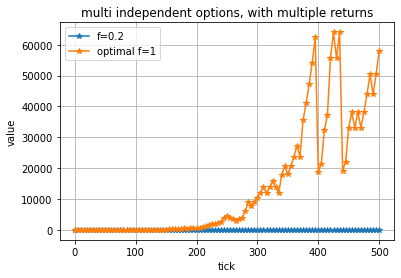
\includegraphics[width=0.9\linewidth]{single1} 
			\label{fig:subim1}
		\end{subfigure}
		\begin{subfigure}{0.525\textwidth}
			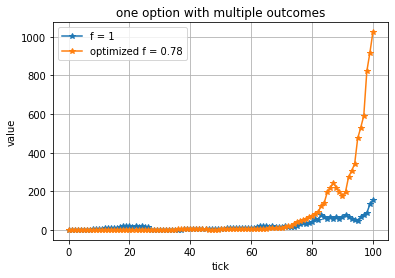
\includegraphics[width=0.9\linewidth]{single2}
			\label{fig:subim2}
		\end{subfigure}
		\caption{Two random simulation with and without optimal value}
		\label{Fig:single1}
	\end{figure}
	
	
	\newpage
	\section{The Expended Model}
	\subsection{Defining The Model}
	The new model will be very similar in some aspects to the Base model, but at the same time different and more robust. The complexity comes from the inclusion of more option with more outcomes so we will be able to calculate more realistic results. In the model each options has it's own distribution and returns and our choice will not be own dimensional, but multidimensional, meaning we will need to know how to split our cash each round between not-investing and all of the options together.\newline
	In order to actually start talking about the returns, we will need to define our fortune at each round.\\
	\begin{equation}
	\label{multi-dim-fortune}
	F_N = \Bigg\{
	\begin{aligned}
		&(b + \overrightarrow{a}\cdot \overrightarrow{f})F_{N-1} &&N > 1 \text{, for each posible outcome }\overrightarrow{a}\\
		&1 &&for \enspace N=1
	\end{aligned}
	\end{equation}
	Unlike in the previous model where each outcome was simply a real number, here it is a vector of real numbers representing the return of all the options (returns can be $0$ if the option didn't win at all or even negative if the loss was high enough)
	in the vector the $i$-th element represent the return of $i$-th option.
	\\
	However if an option did win but we didn't invest in it, the value of the $i$-th element in $\overrightarrow{f}$ would be $0$ meaning it will not be taken into account in calculation of the return.
	\newline
	The only thing left to define is the probabilities in the joint distributions of the options,
	sadly finding the joint distribution is not a simple task, to produce the joint distribution from the probabilities of each option alone. so from now on we will assume that the options are independent from one another in order to simplify the calculation of the joint probability, we will denote the random vector as $X$ with $l$ coordinates so that each $X_i$ would denote the $i$-th random variable corresponding the the $i$-th option inside of  $X$:
	\begin{equation}
		\label{mul-prob}
		P(X = \overrightarrow{\alpha}) = \prod_{i = 1}^l P(X_i = \alpha_i)
	\end{equation}
	After defining both the probability of each outcome (eq.\ref{mul-prob}) and the value at each round (eq.\ref{multi-dim-fortune}) we can create a working Monte-Carlo simulation, However that's not all.\\
	As before I would like to propose the big question: is there an optimal money distribution that would provide the best gains in the long run?\\
	Turns out, there is, but in order to understand why it would take a bit more.\\
	in order to find such a distribution we will define a non-linear optimization problem that we would need to solve in order to find it.\\
	Looking at eq.\ref{exp:FN} as reference I would like to expend it in order to find the gain at $\infty$ for our current model.
	\newpage
	The group $S_l$ is the Probability space:
	\[S_l = \left\{\overrightarrow{a}|\overrightarrow{a} \in \mathbb{R}^l, \text{ for every vector } \overrightarrow{a} \text{ of possible outcome for the } l \text{ options} \right\}\]
	\begin{equation}
		\label{multi:gain}
		G(\overrightarrow{f}) = \lim_{N \to \infty} \frac{1}{N}\log(\frac{F_N}{F_0}) = \sum_{\overrightarrow{a} \in S_l} P(X=\overrightarrow{a})\log(b + \overrightarrow{f} \cdot \overrightarrow{a} )
	\end{equation}
	In this model we have $l$ options total,the $i$-th option have $k_i$ outcomes, however that is not the end, we have to constrain $\overrightarrow{f}$ in order to insure that we don't distribute more money then we have, and each fraction is a positive part of our overall, money.
	making it a maximization problem on a simplex.
	\newline \newline
	\textbf{Maximize:} \[
		G(\overrightarrow{f}) = \sum_{\overrightarrow{a} \in S_l} P(X=\overrightarrow{a})\log(b + \overrightarrow{f} \cdot \overrightarrow{a} )
		\]
	\textbf{s.t:}
	\[
	\begin{aligned}
		&b + \sum_{i=1}^{l} f_i = 1\\
		&f_i \ge 0 \text{, for } i=1..l
	\end{aligned}
	\]
	solving this NLP problem is not an easy task, which would require calculating very big system of Lagrangian multipliers, however before trying to actually solve the system I would like to make a few statements.
	\begin{thm}
		$G(f)$ (eq.\ref{multi:gain}) is a concave function in the non-negative part of $\mathbb{R}^l$.
	\end{thm}
	\begin{proof}
		In order to prove that $G(f)$ is concave, I will prove that $-G(f)$ is convex.\\
		So let's look at each component of of the sum, and prove that it is convex
		\[
		\begin{aligned}
			&&C_{\overrightarrow{a}}(f) = -\log(b + \overrightarrow{f} \cdot \overrightarrow{a})
		\end{aligned}
		\]
		because $C_{\overrightarrow{a}}(f)$ is a composition of $y(x) = -log(x)$ which is nondecreasing, univariate, convex function with hyperplane which is a convex function, we get that the composition is convex (this property stated in \cite{NLP}),
		and the sum of all $C_{\overrightarrow{a}}(f)$ is convex making $-G(f)$ convex.
		\newline
	\end{proof}
	because $G(f)$ is concave our problem is finding the maximum of a concave function, which grant us couple of things:
	\begin{enumerate}
		\item we know that a maximum point exists in the constraints.
		\item if we use iterative algorithm that converge to a local maxima, we get that the convergence point is in fact the maxima in the constraints.
		\label{adv}
	\end{enumerate}
	because of advantage (\ref{adv}) I decided to solve the optimization problem by using an algorithm called \textit{SLSQP}\cite{SQP}\cite{Scipy}\cite{matlab}
	(Sequential Least SQuares Programming) which aims to find a local minima in the feasible set, so I first changed the problem to a minimization problem in order to use SLSQP:
	\newpage
	\textbf{Minimize:}
	 \[
	H(\overrightarrow{f}) = -\sum_{\overrightarrow{a} \in S_l} P(X=\overrightarrow{a})\log(b + \overrightarrow{f} \cdot \overrightarrow{a} )
	\]
	\textbf{s.t:}
	\[
	\begin{aligned}
		&b + \sum_{i=1}^{l} f_i = 1\\
		&f_i \ge 0 \text{, for } i=1..l
	\end{aligned}
	\]
	but because it is a convex minimization problem, which insures that the local minima is the global minima and it exists in the feasible set, which is important because SLSQP solution converges to a local minima, which in our case, would be the optimal solution.
	\newline
	Sequential Quadratic Programming that is used in SLSQP is a way to solve the KKT equations using constrained quasi-Newton methods that guarantee superlinear convergence by accumulating second-order information regarding the KKT equations, since QP subproblems are solved at each major iterations.
	\newline\newline
	It is important to note that running the SLSQP algorithm to find the optimal fraction was extremely fast, which is very assuring if this work will become the basis for an actual trading bot, which would need fast runtime in order to trade in high frequency which is very ideal according to \cite{Feng8388} and its sources.
	\subsection{The Expended Simulations}
	The new simulation holds in memory $l$ tables that represent the distribution of each option and general information like: rounds, $F_0$, $\overrightarrow{f}$ and $b$(fraction of the money that we don't invest). afterwards it runs the model for the amount of rounds defined at the beginning each time picking an outcome from each of the options and calculating the amount of money at each round. at the end of the simulation the simulation returns an array (Numpy array \cite{Numpy}) of all the results we gathered along the way.
	which I then take in order to compile graphs and insights from the Monte-Carlo runs.
	however in order to make the model as general as possible the classes that build the simulations were as general as possible in order to allow flexibility with the amount of options and outcomes, which lead to some difficulties when I needed to use SLSQP, because I needed to create the target function and the constraints which were very large and complicated sums and products, so in order to simplify the coding process I decided to add the $b$ parameter as the first parameter of the vector $\overrightarrow{f}$ which in a way could be described as an option with $100\%$ chance to return $100\%$ of the value (safe option), looking at it in this way helped me produce the target function as the huge sum of all the possibilities and utilize more vector operations which led to faster run-times. I used Numpy as a way to save all the relevent data together in memory to speed the simulation because it allowed for less memory reads overall.\newline
	After creating all the necessary framework and pipelines, I was able to produce a piece of software which is very flexible and able to produce as many different experiments as I wanted without a need to write a lot more code for each one of the new tests I conducted.\newline
	
	if we look at Fig (\ref{Fig:multi1}) we can see four random runs of 3 options each with 2 outcomes, while Fig (\ref{Fig:multi2}) represent a bigger system of 5 options each with 3 outcomes.
	
	\begin{figure}[!h]
		\begin{subfigure}{0.525\textwidth}
			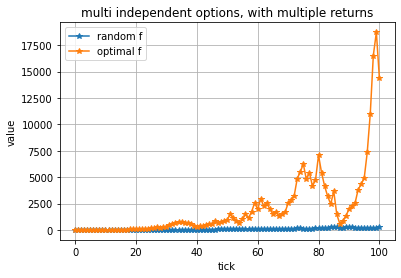
\includegraphics[width=0.9\linewidth]{multi1} 
		\end{subfigure}
		\begin{subfigure}{0.525\textwidth}
			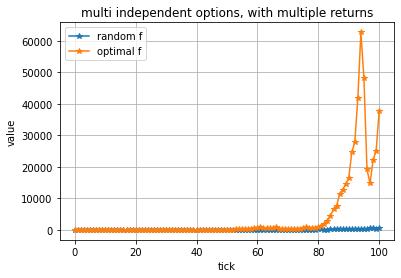
\includegraphics[width=0.9\linewidth]{multi2}
		\end{subfigure}
		\begin{subfigure}{0.525\textwidth}
		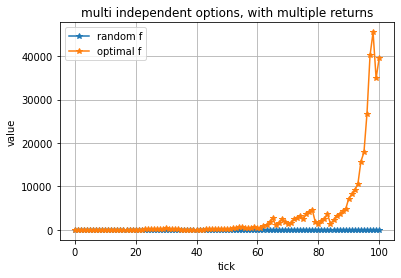
\includegraphics[width=0.9\linewidth]{multi3}
		\end{subfigure}
		\begin{subfigure}{0.525\textwidth}
			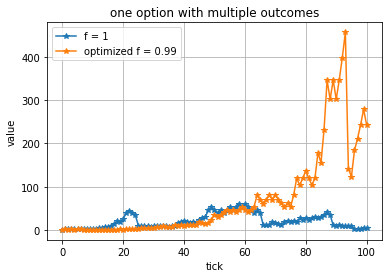
\includegraphics[width=0.9\linewidth]{multi4}
		\end{subfigure}
		\caption{Four random simulation with and without optimal value, 3 options each with 2 outcomes}
		\label{Fig:multi1}
	\end{figure}	

	\begin{figure}[!h]
	\begin{subfigure}{0.525\textwidth}
		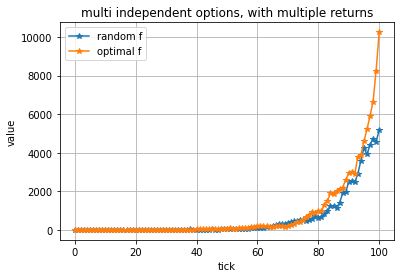
\includegraphics[width=0.9\linewidth]{multi2-1} 
	\end{subfigure}
	\begin{subfigure}{0.525\textwidth}
		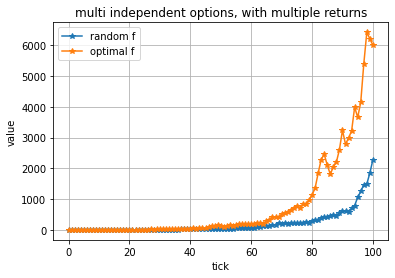
\includegraphics[width=0.9\linewidth]{multi2-2}
	\end{subfigure}
	\begin{subfigure}{0.525\textwidth}
		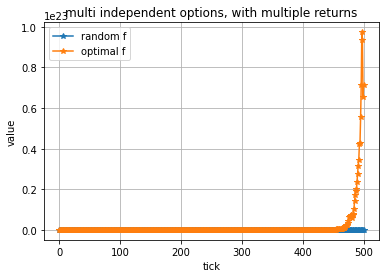
\includegraphics[width=0.9\linewidth]{multi2-3}
	\end{subfigure}
	\begin{subfigure}{0.525\textwidth}
		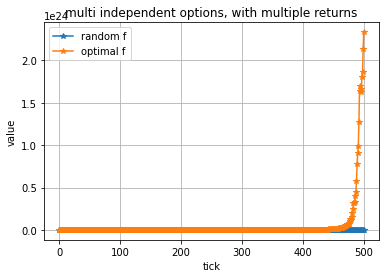
\includegraphics[width=0.9\linewidth]{multi2-4}
	\end{subfigure}
	\caption{Four random simulation with and without optimal value, 5 options each with 3 outcomes}
	\label{Fig:multi2}
\end{figure}
	Because of the random nature of the simulation and the fact that we calculate  the values of $\overrightarrow{f}$ that will produce the best results asymptotically making some simulations that I ran produce results that are countering our statements where the random money distribution produce better results then the optimal one.
	\newpage
	\subsubsection{Example}
	let's look at the following scenario, where we have 5 options, each with the same distribution [Table \ref{prob}] (each produce $E_{gain} \ge 1$) and see what would be the best money distribution in such a scenario:\newline
	
	%% insert probability table
	\begin{table}[!h]
		\centering\begin{tabular}{|c||c|c|c|}
			\hline
			\textbf{probability:} & $0.3$ & $0.5$ & $0.2$ \\ 
			\hline
			 \textbf{gain} & $0.5$ & $1.15$ & $1.5$  \\
			 \hline
		\end{tabular}
	\caption{The outcome of each option in the example}
	\label{prob}
	\end{table}
	
	and the optimal value we got from the SLSQP is 
	\begin{math}
		\overrightarrow{f} = 
		\begin{pmatrix}
			0.1666 \\
			0.1666 \\
			0.1666 \\
			0.1666 \\
			0.1666 \\
			0.1666 \\
		\end{pmatrix}
	\end{math}.
	\newline\newline
	Which could be surprising considering that all of the options are the same, and could have led us to believe that maybe even if had many options that are similar to each other we should have invested only in one or a couple of them, however it turns out that it's the best to stretch our investments over all of them instead of only a couple of them.\\
	\textbf{Note:} this simulation is only a single case, and more work should be put into this question in order to make an absolute statement about similar option.
		\begin{figure}[!h]
		\begin{subfigure}{0.525\textwidth}
			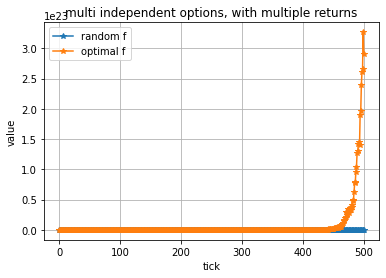
\includegraphics[width=0.9\linewidth]{example1} 
		\end{subfigure}
		\begin{subfigure}{0.525\textwidth}
			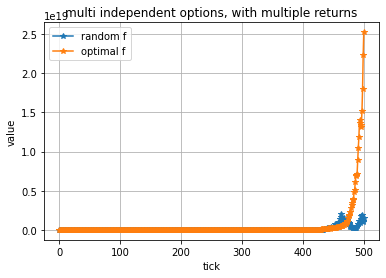
\includegraphics[width=0.9\linewidth]{example2}
		\end{subfigure}
		\caption{Two simulations for the example with random and optimal values}
		\label{Fig:example1}
	\end{figure}
	\section{Summery and conclusions}
	Kelly's criterion can be viewed as a simplified game of chance with a very powerful massage, 
	\textbf{don't stretch yourself too thin}, the model gives us clues into the world of investments where we could sometimes win and sometimes lose, but with the ideas of mitigating losses and long term involvement, instead of looking to quick gain. We look at the long run by cutting future losses and making sure that when we lose, we won't loss all of our savings, but as a trade off when we gain we will not gain a well as we could have.\\
	When we look at the expended model we learn that splitting our money between similar investments is a good way to go, further enforcing the idea that the poor gets poorer and the rich richer, because they have much more "gas" to stretch themselves instead of just looking for quick gains. In addition the expended model at least to my own testing runs very fast which is reassuring because if this work would be the basis of a trading bot that would implement a strategy to invest in multiple options, it would be very beneficial that the bot would be fast agile, which would enable it to trade in high frequency instead of a more fundamental approach in order to maximize the gain it would have otherwise lost because of the money split.
	\newpage
	\printbibliography[
	heading=bibintoc,
	title={References}
	]
\end{document}